\documentclass[sigconf,10pt]{acmart}

\usepackage[english]{babel}
\usepackage{booktabs}
\usepackage{multirow}
\usepackage{xcolor}
\usepackage{balance}
\emergencystretch=1.5em

% Copyright
\renewcommand\footnotetextcopyrightpermission[1]{}
\setcopyright{none}

\settopmatter{printacmref=false, printccs=false, printfolios=true}

\acmDOI{}
\acmISBN{}
\acmPrice{}
\acmConference{CS244C}{Winter 2026}{Stanford, California}

\begin{document}
\title[Generalization in Learned Congestion Control]{Generalization in Learned Congestion Control:\\Decision Trees, Deep RL, and LLM-Guided Evolution}

\author{Duy Nguyen}
\affiliation{%
  \institution{Stanford University}
}
\email{duynguy@stanford.edu}

\author{Andrew Grant}
\affiliation{%
  \institution{Stanford University}
}
\email{agrant27@stanford.edu}

\author{Armaan Abraham}
\affiliation{%
  \institution{Stanford University}
}
\email{armaana@stanford.edu}

\renewcommand{\shortauthors}{Nguyen, Grant, Abraham}

\begin{abstract}
Remy~\cite{winstein2013tcp} showed that computer-generated congestion control
algorithms can outperform human designs within their training distribution, but
generalize poorly outside it. Despite this being known for over a decade, no
one has put alternative representations on Remy's generalization graphs under
the same setup: same observations, same actions, same environments.

We add two new lines. Training a PPO neural network and AlphaCC (an
LLM-guided code evolution system) on a single condition (10~Mbps, 150~ms RTT,
2~senders), we evaluate across a 1000$\times$ range of link rates.
\textbf{Representation matters}: Remy peaks near training (best at 3/9 rates)
but degrades sharply at both extremes; PPO degrades more uniformly but is
worse than Remy at all~9 rates; AlphaCC is best at 5/9 rates (high link
rates), with the flattest degradation curve---yet no method dominates
everywhere. We also run 12~independent AlphaCC evolution runs from
4~structurally different seed families: all~12 converge on the same
interpretable design (in-flight-proportional scaling and rate-based pacing),
suggesting the LLM's TCP prior strongly constrains search. Despite this
reliable mechanism discovery, no systematic run surpasses Remy on the
aggregate mean.
\end{abstract}

\maketitle

\section{Introduction}

Remy~\cite{winstein2013tcp} demonstrated that computer-generated congestion
control algorithms could outperform decades of human design within their
training distribution. However, Remy's decision tree CCAs generalize poorly
to network conditions outside their training range. Despite this being identified over a decade ago, to our knowledge no
prior work has placed alternative representations on Remy's
generalization graphs---training on the same environments, with the
same observation and action spaces.

We set out to add new lines to these graphs. Keeping the observation space
(4~EWMA features) and action space (window\_increment, window\_multiple,
intersend) fixed, we ask: \textbf{how do a neural network and an LLM-guided
code evolution system compare to Remy's decision trees on
out-of-distribution generalization?}

We compare three representations:

\begin{enumerate}
\item \textbf{Decision trees} (Remy): A WhiskerTree maps observation bins to
  actions, optimized by evolutionary search over tree structure.
\item \textbf{Neural networks} (PPO): A neural network maps the same observations
  to the same actions, trained by
  proximal policy optimization (PPO) \cite{schulman2017ppo} in Remy's C++ simulator.
\item \textbf{Source code} (AlphaCC): An LLM (GPT-5.3-codex) generates
  Python functions mapping observations to actions, evolved by
  mutation with simulation-based fitness.
\end{enumerate}

The third paradigm was not part of the original plan. We added it after
observing that PPO generalizes surprisingly well, and were curious
whether an approach
that produces \emph{readable code}---rather than opaque weights---would
generalize differently. The answer is surprising: across 12 independent
evolution runs from 4 seed families (constant, AIMD, Copa, pacing), the method
repeatedly rediscovered the same interpretable rate-aware
design---BDP-proportional scaling and rate-based pacing---regardless of the
starting point (12/12 convergence). However, the best systematic run ($-$1.40)
only approached, and did not surpass, Remy ($-$1.35) on the aggregate 9-rate
mean, indicating reliable mechanistic convergence without a robust
performance win.


%% ====================================================================
%% METHODS
%% ====================================================================
\section{Methods}
\label{sec:methods}

%% ====================================================================
%% ANDREW'S SECTIONS: Remy Framework + Simulator Calibration
%% ====================================================================
\subsection{Simulation Setup and Evaluation}

\paragraph{Simulation setup.}
We use the same dumbbell network topology as in Remy \cite{winstein2013tcp}, consisting of two senders which randomly start and stop flows. Each flow's duration is sampled from an exponential distribution, and during a flow a sender chooses when and how many packets to send. For each set of CCAs we evaluate, this decision of whether to send a packet at a given time is determined by the congestion window and the minimum time interval between sent packets, and these are directly updated by the action chosen by each policy. To compare the generalization of each CCA learning scheme, we fix all network conditions of the simulator except for the link rate, which we vary in both the learning and evaluation process. These 

% TODO(Andrew): Write this section. Cover:
% - WhiskerTree structure (observation = 4 EWMAs, action = 3-tuple)
% - Observation space: send_ewma, rec_ewma, rtt_ratio, slow_rec_ewma
% - Action space: window_increment, window_multiple, intersend
% - Utility function: U = log2(throughput) - delta * log2(delay), delta=1
% - ConfigRange and how Remy trains
% - Learnability paper trees (1x, 10x, 20x, 1000x) and what they mean
%
% Keep the following shared definitions (other sections reference them):

\paragraph{Normalized score.}
To compare across link rates, we use a normalized score:
\begin{equation}
S = \log_2\!\left(\frac{\text{throughput}}{\text{capacity}}\right) - \log_2\!\left(\frac{\text{delay}}{\text{min\_rtt}}\right)
\end{equation}
This measures how close a CCA comes to fully utilizing the link (first term)
while keeping delay near the propagation minimum (second term). A score of 0
means perfect utilization with zero queuing delay. All results report
mean $\pm$ standard deviation across 5 random seeds unless noted.



Remy, PPO, and AlphaCC are each trained on a single condition: 1.5~packets/ms
link rate ($15~Mbps), 150~ms propagation RTT, 2 senders with
Poisson on/off traffic (mean 1s on, 1s off). We additionally extend
AlphaCC to multipoint training on 6 link rates spanning Remy 10x's
range (\S\ref{sec:diverse_seeds}) to study mechanism convergence.
All evaluations use this same traffic model.

\paragraph{Evaluation protocol.}
Primary evaluation: 50 log-spaced link rates from 1--1000~Mbps
(\texttt{np.logspace($-$1, 2, 50)} packets/ms), matching the density and
range of Remy's original generalization plots~\cite{winstein2013tcp}.
RTT${}={}$150~ms, 2 senders. Simulation duration scales inversely with
link rate (30s at low rates, 5s at $>$100~Mbps) to keep wall-clock time
bounded while ensuring at least 33~RTTs of traffic at every rate.
Extended evaluation: 3 RTT values (50, 150, 300~ms) $\times$ 2 link rates
(9.5 and 59.8~Mbps).
Remy is a single deterministic tree (variance from sim seeds only);
PPO std is across 6 independently trained brains; Copa, AIMD, and
AlphaCC std are across 5 sim seeds.

\paragraph{Comparison summary.}
The three methods share the same observation space (4 EWMAs), action
space (window increment, multiplier, intersend), and evaluation protocol,
but differ along other axes (Table~\ref{tab:fairness}).

\begin{table}[t]
\centering
\caption{Method comparison: shared setup and differences.}
\label{tab:fairness}
\small
\setlength{\tabcolsep}{4pt}
\begin{tabular}{@{}llll@{}}
\toprule
 & Remy & PPO & AlphaCC \\
\midrule
\textit{Representation}  & Decision tree     & Neural net (5K)   & Python source     \\
\textit{Optimizer}        & Tree search       & Proximal policy   & LLM evolution     \\
\textit{Simulator}        & C++ (original)    & C++ (original)    & Python (reimpl.)  \\
\textit{Statefulness}     & Stateless         & Stateless         & Stateful          \\
\bottomrule
\end{tabular}
\end{table}

\subsection{Simulator Calibration}
\label{sec:calibration}

% TODO(Andrew): Write this section. Cover:
% - Python reimplementation of Remy's C++ event-driven simulator
% - Per-tick event ordering, single-packet-per-sender-per-tick semantics
% - WhiskerTree protobuf parsing and cross-simulator validation
% - Results: 2 tree sizes x 9 link rates, mean error 2.9%, max 10.9%
% - PRNG differences (Python vs C++ Mersenne Twister)
% - Calibration figure (figures/calibration.pdf exists)
% - Learnability tree evaluation methodology

%% ====================================================================
%% ARMAAN'S SECTION: Deep RL Methodology
%% ====================================================================
\subsection{PPO: Deep Reinforcement Learning}
\label{sec:ppo}

% TODO(Armaan): Expand with architecture details, hyperparameters,
% and analysis of PPO's strong generalization.
We refactored Remy's C++ simulator to expose a gym-like interface and trained
a PolicyNet (${\sim}$5000 parameters) using proximal policy optimization.
The network maps the same 4D EWMA observations to discretized actions via
three categorical heads (257/101/56 classes for window\_increment,
window\_multiple, and intersend respectively). We trained 6 independent runs
(``brains'') to measure training variance.

\subsection{AlphaCC: LLM-Guided Code Evolution}
\label{sec:alphacc}

\subsubsection{Evolution Architecture}

Our approach adapts LLM-guided code evolution, inspired by
AlphaEvolve~\cite{alphaevolve2025}, to congestion control. The evolution loop
proceeds as follows:

\begin{enumerate}
\item \textbf{Seed population}: We initialize with hand-designed CCAs
  implemented as Python functions. For single-point training: AIMD, Copa, an
  adaptive hybrid, and a BBR-like estimator. For the diverse-seed study:
  constant (minimal), AIMD, and pacing seeds (\S\ref{sec:diverse_seeds}).
\item \textbf{Mutation}: GPT-5.3-codex receives the parent policy's source
  code, its fitness score, and the top-performing policies in the archive.
  It generates a mutated policy.
\item \textbf{Evaluation}: The candidate is compiled, sanity-checked (it must
  increase the congestion window when no congestion is detected), and evaluated
  on the training condition.
\item \textbf{Selection}: Parents are chosen with 50\% exploitation (highest
  fitness) and 50\% exploration (random archive member).
\end{enumerate}

We run 15 generations with 5 candidates per generation (75 total evaluations
for single-point; 150 for multipoint across 6 rates).

\subsubsection{Policy Representation}

AlphaCC policies are Python functions with the signature:
\begin{verbatim}
def evolved_policy(obs) -> action
\end{verbatim}
where \texttt{obs} is Remy's Memory (4 EWMAs) and \texttt{action} is Remy's
Action triple (window\_increment, window\_multiple, intersend). Policies can
maintain state across calls via function attributes (e.g.,
\texttt{evolved\_policy.phase}), enabling stateful behaviors like phase
transitions and bandwidth estimation.

Note that AlphaCC policies can maintain arbitrary state across calls via
function attributes, which is additional representational power not available
to Remy's stateless tree mapping or PPO's feedforward network. The
statefulness ablation (\S\ref{sec:ablation}) partially addresses this
confound.


%% ====================================================================
%% RESULTS
%% ====================================================================
\section{Results}
\label{sec:results}

\subsection{Main Comparison: All Methods Across Link Rates}
\label{sec:main_comparison}

Figure~\ref{fig:generalization} shows the normalized score for all methods
across 50 log-spaced link rates from 1--1000~Mbps, matching the density and
range of Remy's original evaluation. Table~\ref{tab:generalization} reports
scores at 9 representative link rates for precise comparison.

\begin{figure*}[t]
\centering
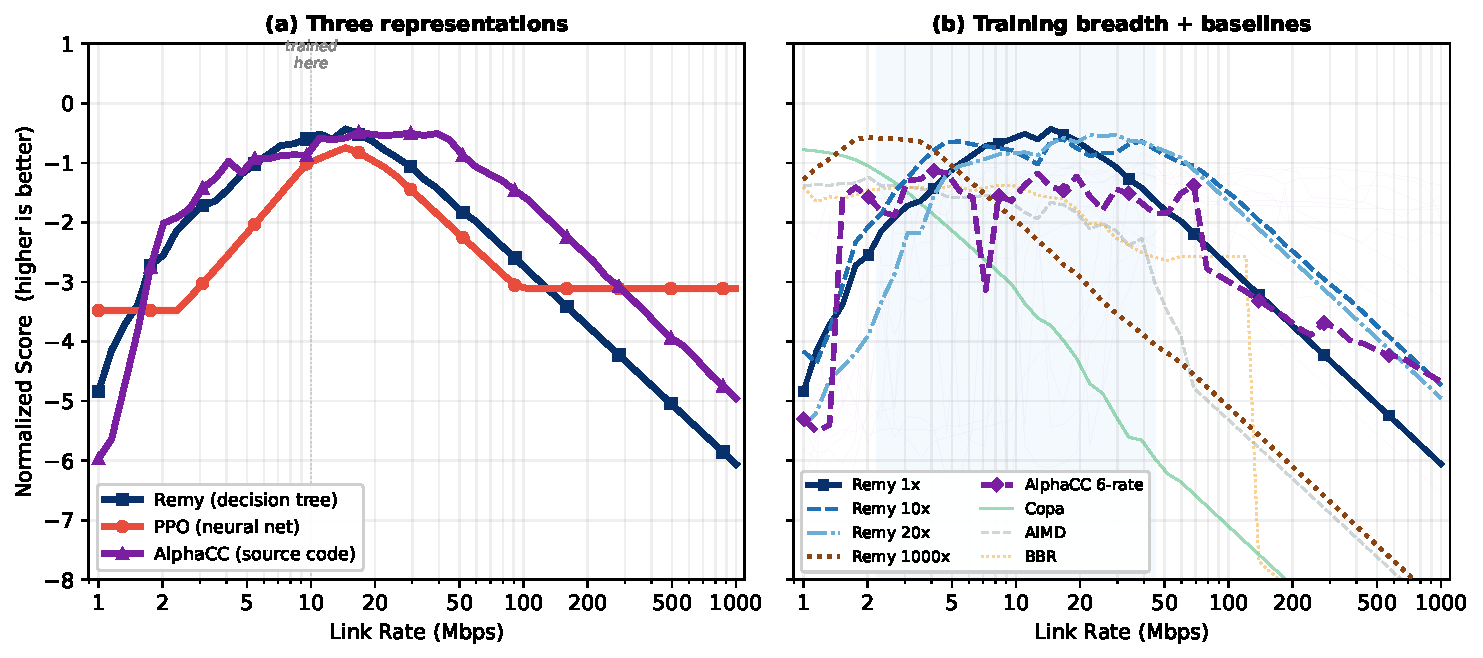
\includegraphics[width=\textwidth]{figures/generalization}
\caption{(a)~Three representations trained at 10~Mbps. (b)~Effect of training breadth and hand-designed baselines.}
\label{fig:generalization}
\end{figure*}

\begin{table*}[t]
\centering
\caption{Normalized score across 9 link rates. Bold = best. All learned methods trained at 10~Mbps; AlphaCC-6pt trained on 6 rates.}
\label{tab:generalization}
\small
\setlength{\tabcolsep}{6pt}
\begin{tabular}{@{}rrrrrrrr@{}}
\toprule
Mbps & Remy & PPO & Copa & AIMD & BBR & \multicolumn{1}{c}{\shortstack{Alpha\\CC-1pt}} & \multicolumn{1}{c}{\shortstack{Alpha\\CC-6pt}} \\
\midrule
2.4  & $-$2.16 & $-$1.74{\scriptsize$\pm$.03} & \textbf{$-$1.36}{\scriptsize$\pm$.10} & $-$1.45{\scriptsize$\pm$.08} & $-$1.79{\scriptsize$\pm$.73} & $-$1.89 & $-$1.30 \\
3.8  & $-$1.55 & $-$1.34{\scriptsize$\pm$.05} & $-$1.83{\scriptsize$\pm$.10} & $-$1.46{\scriptsize$\pm$.07} & $-$1.75{\scriptsize$\pm$.72} & \textbf{$-$1.13} & $-$1.15 \\
6.0  & \textbf{$-$0.91} & $-$0.93{\scriptsize$\pm$.03} & $-$2.42{\scriptsize$\pm$.11} & $-$1.62{\scriptsize$\pm$.10} & $-$1.77{\scriptsize$\pm$.71} & $-$0.93 & $-$1.34 \\
9.5  & $-$0.60 & \textbf{$-$0.51}{\scriptsize$\pm$.02} & $-$3.06{\scriptsize$\pm$.12} & $-$1.81{\scriptsize$\pm$.14} & $-$1.72{\scriptsize$\pm$.66} & $-$0.87 & $-$1.10 \\
15.0 & $-$0.40 & \textbf{$-$0.36}{\scriptsize$\pm$.01} & $-$3.71{\scriptsize$\pm$.12} & $-$1.82{\scriptsize$\pm$.12} & $-$1.70{\scriptsize$\pm$.66} & $-$0.56 & $-$1.73 \\
23.8 & $-$0.80 & $-$0.57{\scriptsize$\pm$.02} & $-$4.37{\scriptsize$\pm$.12} & $-$2.08{\scriptsize$\pm$.19} & $-$1.67{\scriptsize$\pm$.69} & \textbf{$-$0.54} & $-$1.45 \\
37.7 & $-$1.26 & $-$0.90{\scriptsize$\pm$.01} & $-$5.03{\scriptsize$\pm$.12} & $-$2.28{\scriptsize$\pm$.21} & $-$2.17{\scriptsize$\pm$.67} & \textbf{$-$0.52} & $-$1.28 \\
59.8 & $-$1.92 & $-$1.23{\scriptsize$\pm$.01} & $-$5.70{\scriptsize$\pm$.12} & $-$2.37{\scriptsize$\pm$.20} & $-$2.40{\scriptsize$\pm$.85} & \textbf{$-$1.07} & $-$1.43 \\
94.9 & $-$2.59 & $-$1.56{\scriptsize$\pm$.02} & $-$6.36{\scriptsize$\pm$.12} & $-$2.65{\scriptsize$\pm$.35} & $-$2.56{\scriptsize$\pm$.88} & \textbf{$-$1.51} & $-$1.81 \\
\bottomrule
\end{tabular}
\end{table*}

Remy~1x peaks near training (10~Mbps) but degrades sharply at both
extremes, reproducing the overfitting pattern from the original
paper~\cite{winstein2013tcp}. The broader Remy 10x and 20x trees
trade peak performance for wider coverage but still degrade outside
their training ranges. We also evaluate Remy 1000x from the
Learnability study~\cite{sivaraman2014experimental}, trained on
1--1000~Mbps: despite maximal breadth, it underperforms Remy 10x
above 5~Mbps, suggesting that wider training ranges do not
monotonically improve generalization in our simulator.

Among single-training-point methods, AlphaCC achieves the best score at
5 of 9 evaluation rates (4 above 22~Mbps plus 3.6~Mbps), outperforming both PPO and
Remy at high rates (Table~\ref{tab:generalization}). PPO is best at 2
rates near training (9.5 and 15~Mbps) and degrades more gracefully than
Remy~1x, beating it at 8/9 rates. Single-point AlphaCC peaks near
training like Remy~1x but degrades less steeply, maintaining scores
above $-$1.1 through 60~Mbps. At high rates ($>$37~Mbps), Remy 10x
and 20x still outperform PPO (Figure~\ref{fig:generalization}),
reflecting their wider training ranges.

%% ====================================================================
%% ARMAAN'S SECTION: PPO Ablations
%% ====================================================================
\subsection{PPO Ablations}
\label{sec:ppo_ablation}

% TODO(Armaan): PPO-specific ablations go here.
% Possible subsections:
% - Score over training time
% - Comparison against larger network
% - Hyperparameter sensitivity

\subsection{Multipoint Training and Diverse-Seed Evolution}
\label{sec:diverse_seeds}

To test how AlphaCC responds to additional environmental feedback, we
extended it to multipoint training across 6 link rates (matching
Remy 10$\times$'s training range), with 15 generations, 5 candidates
per generation, and per-rate feedback in the prompt.

To test whether AlphaCC's key mechanisms emerge reliably or are artifacts
of lucky initialization, we designed a controlled experiment using four
seed families that span the space of CCA architectures:
\begin{itemize}
\item \textbf{Constant}: minimal seed (increment=1, multiple=1.0,
  intersend=0). The LLM must discover all congestion-control structure.
\item \textbf{AIMD}: additive-increase multiplicative-decrease with
  basic RTT-ratio thresholds. Classical loss-based structure.
\item \textbf{Copa}: delay-based seed using RTT-ratio thresholds.
  Increase when below target, decrease when above.
\item \textbf{Pacing}: rate-based seed using \texttt{rec\_ewma} for
  bandwidth estimation and explicit intersend pacing.
\end{itemize}
Each seed was run 3 times independently (different random seeds),
yielding 12 total evolution trajectories. Table~\ref{tab:diverse_seeds}
summarizes the results.

\begin{table}[t]
\centering
\caption{Diverse-seed results (12 runs, 4 families). $\Delta$ = run mean $-$ Remy mean. IFS/Phase: mechanism presence. All 12 use rate-based pacing.}
\label{tab:diverse_seeds}
\footnotesize
\begin{tabular}{@{}llrrccc@{}}
\toprule
Run & Family & Mean & $\Delta$ & Won & IFS & Phase \\
\midrule
pac\_r1   & pacing   & $-$1.40 & $-$0.05 & 4/9 & \checkmark & \checkmark \\
copa\_r3  & copa     & $-$1.41 & $-$0.06 & 3/9 & \checkmark & -- \\
con\_r1   & constant & $-$1.55 & $-$0.20 & 4/9 & \checkmark & -- \\
pac\_r2   & pacing   & $-$1.79 & $-$0.44 & 3/9 & \checkmark & -- \\
con\_r2   & constant & $-$2.15 & $-$0.80 & 1/9 & \checkmark & -- \\
pac\_r3   & pacing   & $-$2.48 & $-$1.12 & 3/9 & \checkmark & -- \\
aimd\_r3  & aimd     & $-$2.51 & $-$1.15 & 2/9 & \checkmark & -- \\
copa\_r1  & copa     & $-$3.04 & $-$1.69 & 1/9 & \checkmark & -- \\
aimd\_r2  & aimd     & $-$3.05 & $-$1.69 & 2/9 & \checkmark & -- \\
con\_r3   & constant & $-$3.33 & $-$1.97 & 2/9 & \checkmark & -- \\
aimd\_r1  & aimd     & $-$3.41 & $-$2.06 & 2/9 & \checkmark & -- \\
copa\_r2  & copa     & $-$3.53 & $-$2.18 & 1/9 & \checkmark & -- \\
\midrule
\multicolumn{2}{l}{\textit{Family medians:}} \\
 & pacing   & $-$1.79 &  &  & 3/3 & 1/3 \\
 & constant & $-$2.15 &  &  & 3/3 & 0/3 \\
 & copa     & $-$3.04 &  &  & 3/3 & 0/3 \\
 & aimd     & $-$3.05 &  &  & 3/3 & 0/3 \\
\bottomrule
\end{tabular}
\end{table}

\textbf{Key findings:}
No systematic run beats Remy on the 9-rate mean. The best (pac\_r1,
$-$1.40) approaches but does not surpass Remy ($-$1.35). The pacing family has the best median ($-$1.79, range 1.08), while AIMD
has the worst median ($-$3.05) though the smallest range (0.90). Copa has the highest variance (range 2.12).

At the highest tested rate (94.9~Mbps), 9/12 runs beat Remy; at 59.8~Mbps,
7/12 beat Remy. Since all 12 runs share in-flight scaling,
this mechanism alone cannot explain the between-run variance; other
factors (coefficient tuning, phase machines) likely determine which
runs succeed at high rates.
Figure~\ref{fig:seed_comparison} shows the distribution of 9-rate means
by seed family.

\begin{figure}[t]
\centering
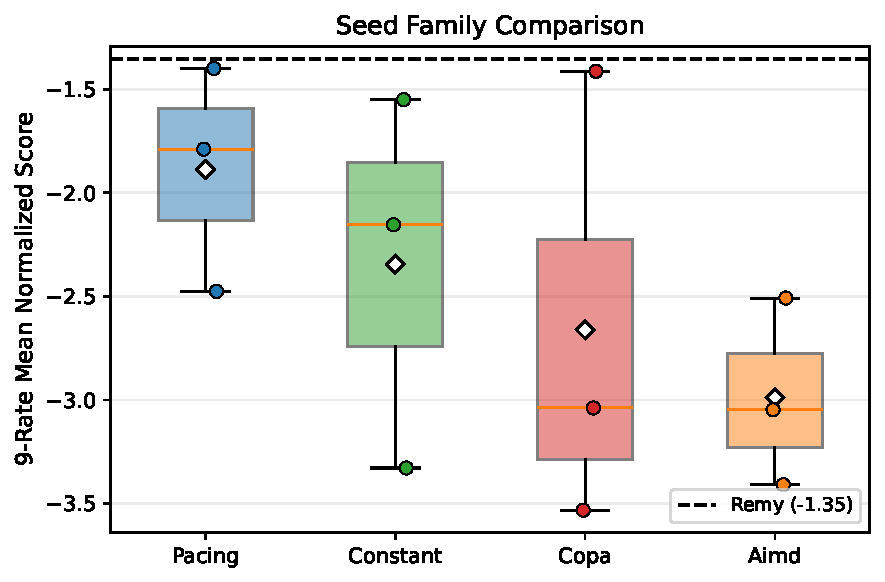
\includegraphics[width=\columnwidth]{figures/seed_boxplot}
\caption{9-rate mean by seed family. Dashed: Remy ($-$1.35).}
\label{fig:seed_comparison}
\end{figure}

\begin{figure}[t]
\centering
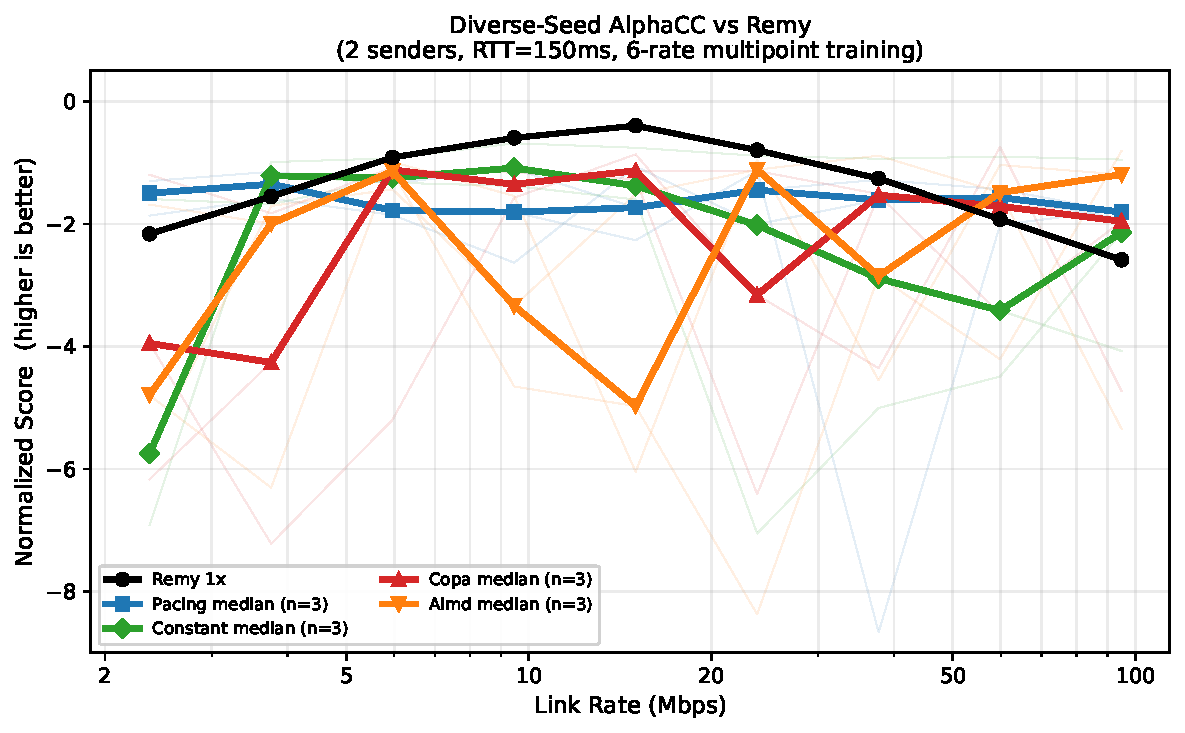
\includegraphics[width=\columnwidth]{figures/seed_lineplot}
\caption{AlphaCC vs Remy across 9 link rates (4 families $\times$ 3 reps). Thick: family medians; faint: individual runs.}
\label{fig:multipoint}
\end{figure}


\subsection{Mechanistic Convergence}
\label{sec:convergence}

The most striking result is not performance but convergence of mechanism.
All 12 evolved policies, regardless of seed family, independently
discovered the same core control structure:

\begin{enumerate}
\item \textbf{BDP estimation}: \texttt{bdp = min\_rtt / rec\_ewma},
  inferring the bandwidth-delay product from the ratio of minimum RTT
  to inter-receive time. Present in 12/12 policies.
\item \textbf{BDP-proportional scaling}: window increments scale with
  $\sqrt{\text{bdp}}$, enabling automatic adaptation to link capacity.
  Present in 12/12 policies.
\item \textbf{Rate-based pacing}: \texttt{intersend} set from
  receive-rate estimates, not purely window-driven. Present in 12/12
  policies.
\item \textbf{Queue pressure sensing}: RTT ratio thresholds
  (${\sim}$1.3 and ${\sim}$2.0) gate transitions between growth,
  maintenance, and backoff. Present in 12/12 policies.
\item \textbf{Phase machines}: explicit startup/drain/steady state
  transitions, analogous to BBR's state machine. Present in 1/12
  systematic runs (pac\_r1).
\end{enumerate}

\paragraph{Mechanism coding methodology.}
We inspected each of the 9 final policies and classified the
presence of five structural elements:
\begin{enumerate}
\item BDP estimation: computing ratio of minimum RTT
  to smoothed receive rate, or equivalent;
\item BDP-proportional scaling: gain proportional to
  $\sqrt{\mathrm{bdp}}$ or similar;
\item Rate-based pacing: \texttt{intersend} set from receive-rate;
\item Queue pressure: RTT-ratio thresholds gating
  growth\slash backoff;
\item Phase machines: explicit state variables for startup,
  drain, and steady states.
\end{enumerate}
Coding was performed by one author post hoc; labels were not used
during evolution.

This convergence is notable because the three seed families encode
fundamentally different CCA architectures: the constant seed provides
\emph{no} congestion-control structure at all (the LLM must invent
everything), AIMD provides loss-based structure, and pacing provides
rate-based structure. That all three converge on the same BDP-scaled
pacing mechanism suggests the LLM's pre-trained knowledge of TCP
strongly biases search toward this design. We cannot distinguish
whether this reflects a genuine attractor in the fitness landscape
or simply the LLM's inability to explore beyond familiar TCP
templates; both explanations are consistent with the data.

Figure~\ref{fig:mechanism} shows the core code excerpted from three
policies evolved from different seed families. Despite different variable
names, smoothing constants, and threshold values, the structural pattern
is identical: estimate BDP from \texttt{min\_rtt / rec\_ewma}, scale
window changes by $\sqrt{\text{BDP}}$, and pace sends at the
estimated receive rate.

Notably, the constant seed provides \emph{zero} congestion-control
structure (increment=1, multiple=1.0, intersend=0), yet the LLM
generated the full BDP-scaling mechanism in its first successful
mutation (generation~1). This is consistent with the LLM importing
a familiar TCP-like template early, after which evolution mainly
tunes parameters and preserves useful structure. However, we cannot
rule out that a different LLM or prompting strategy would discover
qualitatively different mechanisms.

\begin{figure}[t]
\centering
\small
\begin{verbatim}
# From constant_r1 (started from scratch):
bdp_pkts = max(1.0, min_rtt / rec)
scale = max(1.0, min(12.0, math.sqrt(bdp_pkts)))
intersend = 1.0 / max(1e-6, target_rate * pace_gain)
inc = int(max(1.0, round(0.55 * scale + ...)))

# From aimd_r1 (started from AIMD seed):
bdp_est = max(0.2, min(600.0, min_rtt / rec))
bdp_scale = max(1.0, min(18.0, math.sqrt(bdp_est)))
intersend = rec / boost
inc = int(max(1.0, min(36.0, 1.2 + 0.95*bdp_scale)))

# From pacing_r1 (started from pacing seed):
bdp_pkts = max(1.0, min_rtt / rec)
bdp_scale = max(0.7, min(6.0, math.sqrt(bdp_pkts)))
intersend = 1.0 / max(1e-6, target_rate)
inc = max(1, int(1 + 1.4 * bdp_scale))
\end{verbatim}
\caption{Core mechanism from 3 seed families. All compute BDP from min\_rtt/rec\_ewma and pace from receive rate. Structure is identical.}
\label{fig:mechanism}
\end{figure}


\subsection{AlphaCC Ablations}
\label{sec:ablation}

\subsubsection{Pacing Ablation}

Removing \texttt{intersend} (setting to 0) in the single-point best policy
degrades score from $-$0.87 to $-$3.34---catastrophic collapse. In this
ablation, removing pacing eliminates most of the observed advantage over
window-only baselines.

\subsubsection{Statefulness Ablation}

A 10-generation stateless evolution (no function attributes---each call
depends only on current observations) produced a policy scoring $-$2.54
at 9.5~Mbps (near training) and $-$0.75 at 2.4~Mbps
(Table~\ref{tab:ablation}).

\begin{table}[t]
\centering
\caption{Statefulness ablation. AlphaCC: best 3 of 5 exploratory policies
(best 3 of 5 exploratory). Copa: mean $\pm$ std over 5 seeds. Stateless: single evolution
run.}
\label{tab:ablation}
\footnotesize
\begin{tabular}{@{}lrrr@{}}
\toprule
Condition & Stateful & Stateless & Copa \\
\midrule
Near (9.5\,Mbps) & \textbf{$-$0.72}{\scriptsize$\pm$.06} & $-$2.54 & $-$3.06{\scriptsize$\pm$.12} \\
Low (2.4\,Mbps) & $-$1.57{\scriptsize$\pm$.51} & \textbf{$-$0.75} & $-$1.36{\scriptsize$\pm$.10} \\
High (59.8\,Mbps) & \textbf{$-$0.78}{\scriptsize$\pm$.07} & $-$1.92 & $-$5.70{\scriptsize$\pm$.12} \\
\bottomrule
\end{tabular}
\end{table}

\subsubsection{Failure Modes}
\label{sec:failures}

The weaker systematic runs (aimd\_r1 at $-$3.41, constant\_r3 at $-$3.33)
and the prior catastrophic exploratory failures reveal systematic
failure modes:

\begin{enumerate}
\item \textbf{Architectural lock-in}: The seed plus first 3--5 mutations
  determine the policy's architecture (PID controller vs state machine,
  scale cap, coefficient ranges). Subsequent mutations can only tune
  parameters within that architecture---they cannot escape to a
  qualitatively different design.
\item \textbf{Conservative BDP caps}: One failed run committed to
  \texttt{min(16, sqrt(bdp))} early. No local mutation can change the scaling
  law without rewriting the formula. At high BDP ($>$256 packets), the cap
  makes the policy 6$\times$ slower to grow than the winning policies.
\item \textbf{Over-engineering}: Another failed run built a PID-style
  controller with 5+ interacting error terms---too many coefficients for
  30 generations to co-tune.
\item \textbf{Degenerate mutations}: One exploratory run produced mutations
  scoring $-$105 (generation 27). Once evolution falls into a degenerate
  region, AlphaCC has no mechanism to recover.
\end{enumerate}

These failure modes suggest that AlphaCC is fundamentally
\emph{local search}---effective within an architecture, but unable to make the
qualitative jumps needed when the initial architecture is wrong.

\subsubsection{Evolution Trajectory}

Figure~\ref{fig:evolution} shows the trajectory across all 12
diverse-seed runs (4~seed families $\times$ 3~repetitions). Most
improvement occurs in the first 3~generations, with diminishing
returns afterward. The global running best surpasses Remy's
training-condition fitness by generation~2.

\begin{figure}[tbp]
\centering
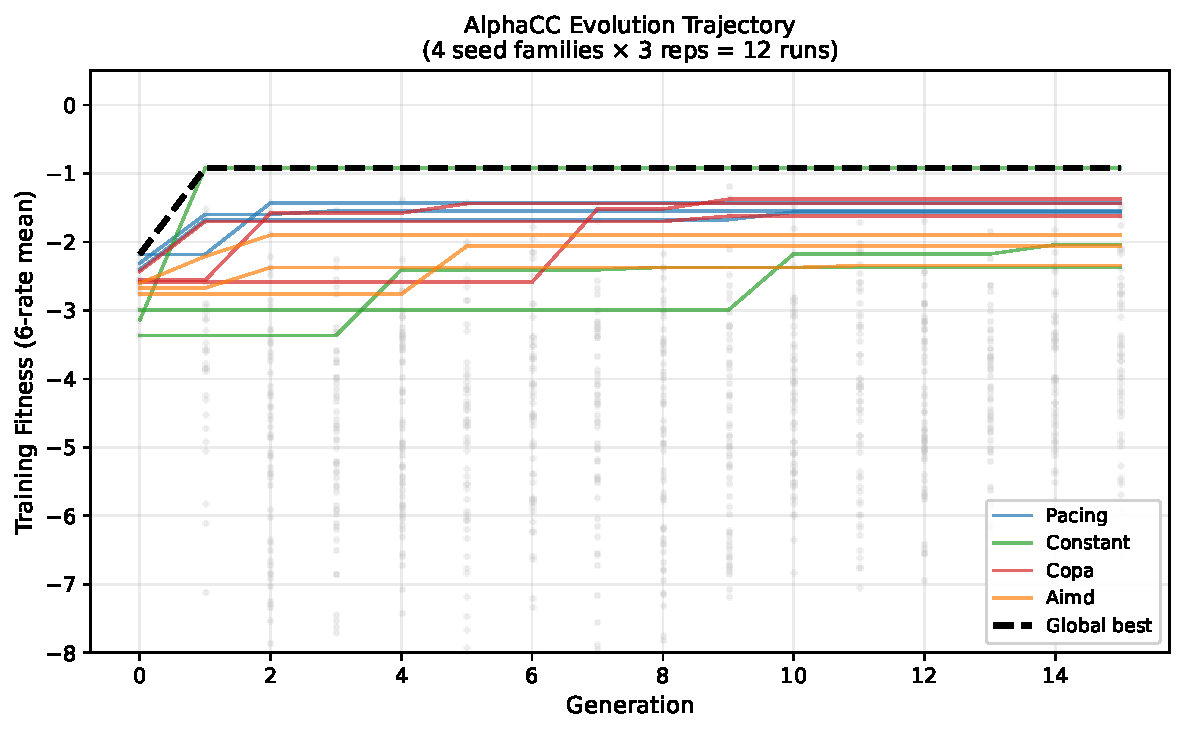
\includegraphics[width=\columnwidth]{figures/evolution_trajectory}
\caption{Evolution trajectory (12 runs, 15 generations). Colored: per-run best by family; black: global best. Most improvement in first 3 generations.}
\label{fig:evolution}
\end{figure}


\subsection{Generalization Across RTT}
\label{sec:rtt}

Figure~\ref{fig:rtt} shows performance for Copa, AIMD, BBR, and AlphaCC
across 3 RTT values $\times$ 2 link rates (6 conditions).
Remy and PPO are omitted because their C++ evaluator does not support
RTT changes at evaluation time. Table~\ref{tab:rtt} reports the scores.

\begin{figure}[tbp]
\centering
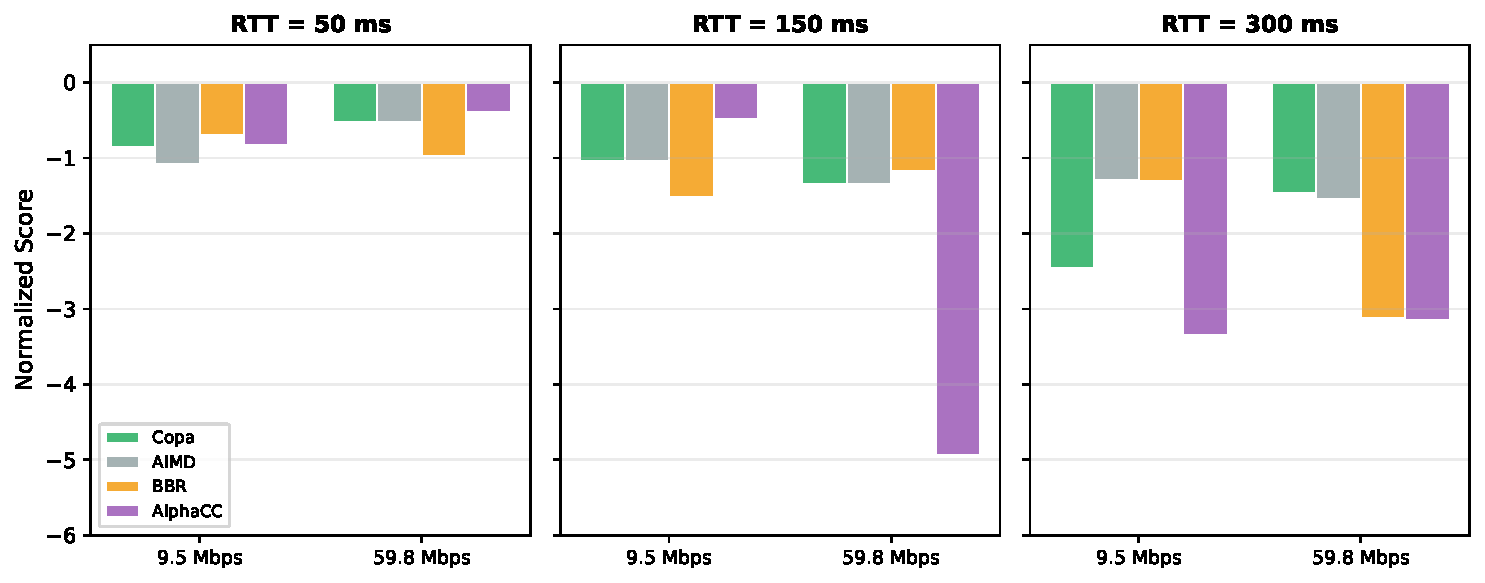
\includegraphics[width=\columnwidth]{figures/rtt_sweep}
\caption{Score across RTT values and link rates. AIMD most consistent; AlphaCC highest variance.}
\label{fig:rtt}
\end{figure}

\begin{table}[tbp]
\centering
\caption{RTT sweep results. Single evaluation per condition. Bold marks the
best score per row.}
\label{tab:rtt}
\small
\begin{tabular}{@{}lrrrr@{}}
\toprule
Condition & Copa & AIMD & BBR & AlphaCC \\
\midrule
50ms, 9.5 Mbps        & $-$0.85 & $-$1.08 & \textbf{$-$0.69} & $-$0.83 \\
150ms, 9.5 Mbps       & $-$1.03 & $-$1.03 & $-$1.52 & \textbf{$-$0.49} \\
300ms, 9.5 Mbps       & $-$2.46 & \textbf{$-$1.29} & $-$1.31 & $-$3.35 \\
50ms, 59.8 Mbps       & $-$0.53 & $-$0.52 & $-$0.98 & \textbf{$-$0.38} \\
150ms, 59.8 Mbps      & $-$1.34 & $-$1.34 & \textbf{$-$1.17} & $-$4.94 \\
300ms, 59.8 Mbps      & \textbf{$-$1.46} & $-$1.54 & $-$3.12 & $-$3.15 \\
\bottomrule
\end{tabular}
\end{table}

AlphaCC achieves the best score ($-$0.38 at 50ms\,/\,59.8~Mbps) but
also the worst ($-$4.94 at 150ms\,/\,59.8~Mbps)---a 4.56-unit swing.
AIMD's range is 1.02 units across the same conditions.


%% ====================================================================
%% DISCUSSION AND RELATED WORK
%% ====================================================================
\section{Discussion}
\label{sec:discussion}

\subsection{What the Comparison Shows}

\textbf{Representation shapes generalization profile.} Each
representation degrades differently outside its training distribution.
Remy~1x overfits tightly to {\sim}10~Mbps and degrades sharply at
both extremes---the original finding of~\cite{sivaraman2014experimental}.
PPO degrades more uniformly but never matches Remy, even near training.
AlphaCC's in-flight scaling adapts window increments to link capacity,
giving it the flattest curve at high rates but losing near training
where Remy's precise tree fit dominates.

\textbf{No method dominates everywhere.} Remy is best near training
(3/9 rates), AlphaCC at high rates (5/9), PPO at none. On the 9-rate
mean, Remy is best ($-$1.35); AlphaCC's best systematic run ($-$1.40)
comes within 3\%. The process is high-variance (means $-$1.40 to
$-$3.53 across 12~runs).

\textbf{PPO underperforms both.} PPO is worse than Remy at all~9
rates despite sharing the same observations, actions, and C++
simulator. We did not conduct a thorough hyperparameter sweep
(6~brains, no architecture search), so we cannot determine whether
this reflects a fundamental limitation of the neural-network
representation or insufficient training.

\textbf{Mechanistic convergence.} All 12~AlphaCC runs converge on
in-flight-scaled pacing regardless of seed family. The most
parsimonious explanation is the LLM's TCP prior:
GPT-5.3-codex was trained on millions of TCP implementations, making
in-flight scaling the path of least resistance. We cannot distinguish
this from a genuine fitness-landscape attractor without a
non-TCP-pretrained LLM (\S\ref{sec:convergence}).

\subsection{Interpretability}

AlphaCC's unique property is human-readable output. The best evolved
policy is 115 lines of Python with named variables and clear control
flow, whereas PPO uses ${\sim}$5000 opaque weights. AlphaCC's output
can be inspected and debugged---enabling the mechanism analysis in
\S\ref{sec:convergence} that would be substantially harder to extract
from a neural network.

\subsection{Limitations}

\begin{enumerate}
\item \textbf{PPO baseline quality}: PPO's strong generalization may partly
  reflect its training setup; further hyperparameter tuning could improve or
  diminish its advantage relative to other methods.
\item \textbf{Simulator mismatch}: Remy/PPO trained in C++;
  AlphaCC trained in Python. Cross-method scores may reflect simulator
  differences as well as representation differences.
\item \textbf{LLM prior vs.\ discovery}: The 12/12 convergence on BDP scaling
  could reflect either (a)~rediscovery of a genuine attractor in the fitness
  landscape or (b)~the LLM's inability to explore beyond familiar TCP
  templates. We cannot distinguish these from simulation alone.
\item \textbf{Small N}: 12 runs (4 families $\times$ 3) provides
  initial evidence for convergence but is insufficient for robust statistical
  claims. Bootstrap CIs and more seeds would strengthen the result.
\item \textbf{No stochastic loss}: All experiments use lossless links.
\item \textbf{Simulator only}: No Mahimahi or real-network validation.

\end{enumerate}


\section{Related Work}

Remy~\cite{winstein2013tcp} pioneered automated CCA design with decision tree
optimization. Sivaraman et al.~\cite{sivaraman2014experimental} studied its
generalization, finding that trees trained on narrow ranges degrade on wider
conditions but that very wide training ranges (1000$\times$) achieve
within-3\% throughput of narrow-range trees.

Several deep RL approaches followed: PCC~\cite{dong2015pcc} used online
learning for utility maximization; Aurora~\cite{jay2019deep} applied deep RL
to congestion control; Yan et al.~\cite{yan2018pantheon} built the Pantheon
benchmarking platform and trained Indigo via imitation learning.
These demonstrated that neural networks can learn congestion control but
did not systematically compare generalization across representations on the
same environments.

CCAC~\cite{arun2021ccac} introduced formal CCA verification using
SMT solvers. CCmatic~\cite{arun2024ccmatic} extended this to automated
synthesis with formal guarantees, but only within a fixed
window-adjustment template.

AlphaEvolve~\cite{alphaevolve2025} demonstrated LLM-guided code
evolution for mathematical optimization. Our approach adapts this
paradigm to congestion control, using simulation-based fitness instead
of mathematical verification.

Copa~\cite{arun2018copa} and BBR~\cite{cardwell2017bbr} represent hand-designed
CCAs that encode domain knowledge about delay-based and model-based congestion
control, respectively.


\section{Conclusion}

We set out to put new lines on Remy's generalization graphs---training
a neural network, an LLM-guided code evolution system, and Remy's
decision trees all on the same single condition (10~Mbps, 150~ms RTT, 2
senders), then evaluating across 1--1000~Mbps. Three findings:

\begin{enumerate}
\item \textbf{Representation shapes generalization.} Remy peaks
  near training (best at 3/9 rates) but degrades sharply at both
  extremes. PPO degrades more uniformly but is worse at all~9
  rates. AlphaCC is best at 5/9 rates (high rates). No method
  dominates everywhere; no systematic AlphaCC run beat Remy on the
  9-rate mean (best: $-$1.40 vs.\ $-$1.35).

\item \textbf{Mechanistic convergence.} Across 12~independent
  AlphaCC runs from 4~seed families, every evolved policy contains
  in-flight-proportional scaling and rate-based pacing (12/12),
  most likely reflecting the LLM's TCP prior rather than a
  fitness-landscape property.

\item \textbf{Reliable mechanism discovery $\neq$ reliable
  performance.} AlphaCC's evolution is high-variance (means
  $-$1.40 to $-$3.53 across 12~runs), and seed family choice
  strongly affects outcome (pacing median $-$1.79 vs.\ AIMD
  $-$3.05).
\end{enumerate}


\balance
\bibliographystyle{ACM-Reference-Format}
\bibliography{reference}

\end{document}
